\section{Specification}
This section aims to inform the reader on the formal project plan that was created for the development of this projects, and the decisions on how it was structured.

\subsection{Development Methodology}
PXP as introduced in the research phase was selected for its well defined (extensively documented in paper) agile based methodology that was well suited to a single-person development team. Agile in general though, was selected over a waterfall technique to allow user feedback to drive design and development which was often collected. The details of the methodology are mainly based on this paper[]
As is a fundamental principle of agile, this methodology was adapted to the project at hand with some main changes being:
\begin{itemize}
    \item No automated testing setup at the start of the project. Graphics development is fairly tricky to automate the testing of as the large majority of testing is completely visual. It is still possible and was considered in section X but was chosen to set aside to rather focus on development and proving that the technology stack was suitable before any more work was committed on it.
    \item Allow refactoring to be raised at any point, also allow grouping of similar user stories to be refactored together. Allowed fixing problems before they became too big and interlinked.
    \item MoSCoW and Cost factors agile ceremonies were considered for the project’s user stories. Allowed better planning and time management.
    \item Instead of tasks created from user stories, user stories themselves are treated like tasks with any non-user story work labelled as tasks instead and treated the same as stories. Done to lower duplication of information.
    \item Reworked development process to better fit the students workflow. See Section S
\end{itemize}

For a more in-depth look into how these changes were implemented and the overall development flow, see section X below

\subsection{Requirements Gathering}
With the goals that the developed application needs to achieve set as per the research phase- The next step was to create a concrete plan on what exact requirements / features would contribute towards achieving those goals. To do that, two main ideas were identified by the student.

The first idea was to conduct Interviews with individuals who commonly use visualization tools or do general data science work. This would provide key insight into what real users of visualization technology think is key for a successful application to have. These requirements would constitute the first phase of the project and set a strong start to either a waterfall type methodology or an agile project.
But there were a couple of downsides that cancelled out this idea at that time:
\begin{itemize}
    \item With no initial product to focus insight into actionable requirements- the interview process is more likely to return conflicting or infeasible requirements.
    \item It might be difficult to offer insight that is not generic for the same reasons. Application should plot data vs Application should do it like this instead of like this. With the latter insight being much more valued.
    \item Time and access to experts is very valuable and needs extensive preparation. It is important to make the most of it, which the student didn’t feel like they could do at that time.
\end{itemize}

The next idea to identify requirements was a two-step process, and one which was inspired by the development methodology chosen to be followed by the student in section X. The student took on the role of the client to create a client brief using the insight gained during the research phase. This brief can be read in full in Appendix A but in short, creates a written source document describing the minimum simplest application that would need to be created. Further improvements would then come from user testing and analysis by the student. The main reason to do this instead of just skipping to creating user stories directly was to have a consistent main source from where user stories were pulled from and were focused on completing the brief's informal requirements.

With a brief set, the next step was to extract user stories (formal requirements) from the brief. Those user stories were all bundled up into an MVP (minimum viable product) feature set which was scheduled as further covered in section X. The specific user stories are all attached in Appendix A.

\subsection{Scheduling}
With a backlog of user stories ready the next step was to combine similar stories into feature sets. Feature sets were then given a deadline on when all of their user stories should be completed.
This would allow then the student to pick the most urgent Feature Set to focus on.

Once a Feature set was picked, each user story and task within was analyzed and given a development time cost and importance to the project. With this, a prioritized backlog was created that was split among the maximum iterations/sprints that would fit into the Feature set's time frame with a consideration for the students iteration velocity. On the off chance that there wasn't enough time to complete all stories and tasks, the student would re-analyze what stories and tasks could be dropped due to time constraints.

Having feature sets allowed the student to put into perspective what are the major additions to the application and if there was enough time to fully develop those additions.

\subsection{Development Flow}
\begin{figure}
    \centering
    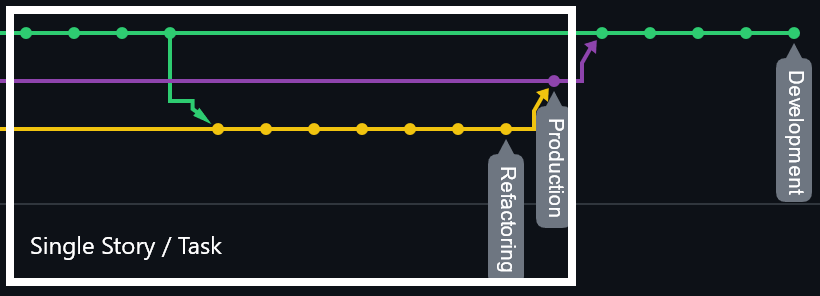
\includegraphics[width=1\columnwidth]{author-files/figures/SingleStoryPath2.png}
    \caption{Development Timeline of a Single Story}
    \label{fig:singlestory}
\end{figure}

Development followed a predefined process where a user story or task was picked to be developed. Once the student has finished developing the one or more tasks picked in the simplest way possible, the student would then push the code to the refactor branch where it would be organized and possibly reworked to follow better practices. This process allowed the student to move fast and encounter obstacles in implementation much more quickly, which minimized the risks of large roadblocks knocking the schedule out of balance. But once the feature was reworked to a sufficient standard with bugs fixed, it was only then pushed to the final Production branch, which was publicly hosted.
This process helped ensure that any code committed to production was vetted and would be unlikely to cause unexpected issues. It also allowed the student to always have a safe version of the application for demos and user testing without having to worry about what work was done before hand.

